\beginsong{Wo's nur Felsen gibt}[wuw={Werner Helwig(1928), nach einem russischen Nomadenlied}, pfii={42}, bo={426}, kssiv={50}, siru={222}]

\beginverse
\endverse
\centering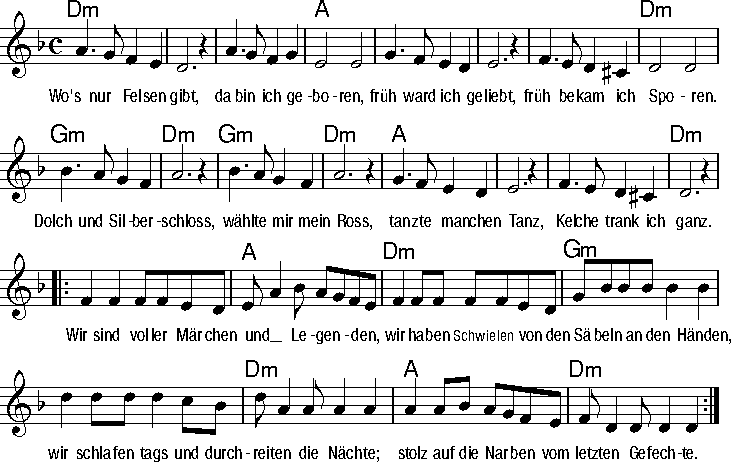
\includegraphics[width=1\textwidth]{Noten/Lied101.pdf}	

\beginverse
\[Dm]Wo im ew'gen Eis stolz der Kasbek \[A]thront, 
hat im stillen Tal einst mein Ahn ge\[Dm]wohnt.
\[Gm]War ein starker \[Dm]Held, \[Gm]kühn und wohlge\[Dm]mut, 
\[A]starb von feindes Hand jäh in seinem \[Dm]Blut.
\endverse

\beginchorus
Wir sind voller Märchen \[A]und Legenden, 
\[Dm]wir haben Schwielen von den \[Gm]Säbeln an den Händen.
Wir schlafen tags und durch\[Dm]reiten die Nächte, 
\[A]stolz auf die Narben vom \[Dm]letzten Gefechte.
\endchorus

\endsong

\beginscripture{}
Der Kasbek ist der drittgrößte Berg Georgiens. Er liegt zwischen dem Schwarzen Meer und dem Kaspischen Meer. Wörtlich bedeutet Kasbek 'Eisgipfel'. 
\endscripture

\begin{intersong}
\ifthenelse{\boolean{pics}}{
    \ThisLRCornerWallPaper{1}{Bilder/wosnurfelsen.jpg}
}{}
\end{intersong}